\section{El algoritmo}
A continuación concretaremos el algoritmo usando la notación de la sección \ref{sec:dnf}. Para optimizar la implementación del algoritmo, se realiza una fase de preprocesamiento en la que calculamos el valor que devolvería un \textit{bad-character-shift} y un \textit{good-suffix-shift} en cualquier situación. Para ello se construyen  dos tablas que concretaremos a continuación:\\

\subsection{Tabla del buen sufijo (GST)}
La primera será denominada la tabla del buen sufijo (GST). Para cada $i$ menor a $m$, construiremos el patrón consistente en los últimos $i$ caracteres de $x$ precedido por un carácter no coincidente con $x$. Es decir, construimos el patrón $c + x[m-1-i \ \ ...\ \ m-1]$ donde $c \neq x[m-2 -i]$ y $+$ representa la concatenación de caracteres. Ahora situaremos el patrón sobre $x$ y anotaremos el número mínimo de posiciones que hemos de mover el patrón a la izquierda para encontrar una coincidencia con $x$.\\

\begin{figure}[H]
  \centering
    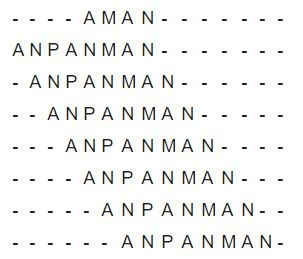
\includegraphics[width=0.45\textwidth]{gst}
  \caption{Tenemos $x[4] = N \neq A$, lo que nos obliga a desplazar $x$ seis caracteres a la izquierda.}
	\label{gst}
\end{figure}

Para la búsqueda de la cadena `ANPANMAN', la tabla sería la siguiente (`\sout{N}MAN' denotará a una cadena compuesta por un carácter diferente de `N' más los carácteres `MAN'): 

\begin{table}[H]
\begin{tabular}{|l|l|l|l|}
\hline
\rowcolor[HTML]{EFEFEF} 
\textbf{i} & \textbf{Patrón} & \textbf{Desp} & \textbf{Explicación}                                                                                                                                                           \\ \hline
0          & \sout{N}               & 1             & \begin{tabular}[c]{@{}l@{}}El penúltimo carácter de $x$ es diferente a `N',\\ con lo que basta desplazar una posición.\end{tabular}                                            \\ \hline
1          & \sout{A}N              & 8             & \begin{tabular}[c]{@{}l@{}}AN no es cadena en $x$ por lo que desplazaremos \\ $m = 8$.\end{tabular}                                                                             \\ \hline
2          & \sout{M}AN             & 3             & \begin{tabular}[c]{@{}l@{}}\sout{M}AN coincide con AN\textbf{PAN}MAN, por lo que \\ desplazamos 3 posiciones.\end{tabular}                                                                     \\ \hline
3          & \sout{N}MAN            & 6             & \begin{tabular}[c]{@{}l@{}}\sout{N}MAN no es subcadena de \textbf{ANPA}NMAN, pero el\\ final de \sout{N}MAN coincide con el inicio de $x$\\ (\sout{NM}\textbf{AN}PANMAN) por lo que desplazamos 6 posiciones.\end{tabular} \\ \hline
4          & \sout{A}NMAN           & 6             & Igual que $i=3$                                                                                                                                                                \\ \hline
5          & \sout{P}ANMAN          & 6             & Igual que $i=3$                                                                                                                                                                \\ \hline
6          & \sout{N}PANMAN         & 6             & Igual que $i=3$                                                                                                                                                                \\ \hline
7          & \sout{A}NPANMAN        & 6             & Igual que $i=3$                                                                                                                                                                \\ \hline
\end{tabular}
\end{table}

El algoritmo originalmente publicado por Boyer y Moore (ver \cite{articulo1}) usa una tabla más simple en la que no se requiere una no-coincidencia para el carácter de más a la izquierda. Sin embargo, esto no es suficiente para conseguir que el algoritmo funcione el tiempo lineal en el peor caso.

\subsection{Tabla del mal carácter (BCT)}
Para calcular esta tabla recorreremos $x$ de derecha a izquierda, empezando por el penúltimo carácter y pasando por todos. Si el carácter en el que nos encontramos no está aún en la tabla, lo añadimos con un desplazamiento asociado igual a su distancia hasta el último carácter. Es decir, si estamos en el carácter $x[i]$, y este aún no figura en la tabla, su desplazamiento asociado será $m - 1 - i$. A los caracteres que no figuren en $x$ se les asignará $m$. Para la cadena `ANPANMAN', la tabla quedaría de esta manera (por claridad, las entradas están ordenadas por orden de inserción): \\ 
 
\begin{table}[H]
\begin{tabular}{|l|l|}
\hline
\rowcolor[HTML]{EFEFEF} 
\textbf{Carácter}    & \textbf{Desplazamiento} \\ \hline
A                    & 1                       \\ \hline
M                    & 2                       \\ \hline
N                    & 3                       \\ \hline
P                    & 5                       \\ \hline
Caracteres restantes & 8                       \\ \hline
\end{tabular}
\end{table}


\subsection{Pseudocódigo}
A continuación se muestra mediante pseudocódigo el funcionamiento del algoritmo de Boyer-Moore (asumimos que tenemos las tablas GST y BCT ya rellenas): 

\begin{algorithm}[H]
\begin{algorithmic}[1]
\caption{Booyer-Moore Algorithm($x,y$)}
\STATE $j = 0$
\WHILE{$j \leq n - m$}
\IF{$x[0\ \ ...\ \ m-1] == y[j\ \ ...\ \ j+m-1]$}
\STATE Hay una coincidencia en $j$, la tratamos como corresponda.
\STATE $j += GST[0]$
\ELSE
\STATE $i =$ Posición en $x$ del primer carácter, contando desde la derecha, en el que difieran $x$ e $y$ ($x[i] \neq y[j + i]$).
\STATE $j += max(GST[i], BCT[y[i + j]] - (m - 1 - i))$
\ENDIF
\ENDWHILE
\end{algorithmic}
\end{algorithm}